% ----------------------------------
% Cap Diseño
% ----------------------------------
%	Incluye
%		Diseño de interfaces y prototipos
%	    
%
\documentclass[a4paper,oneside,11pt]{book}

\usepackage[spanish,activeacute]{babel}
\usepackage[utf8]{inputenc}
%\usepackage[T1]{fontenc}
\usepackage{tabulary}
\usepackage{graphicx}

\usepackage{float}

\setcounter{secnumdepth}{3}

\oddsidemargin=0.2cm
\headsep=1cm
\textheight=21cm
\textwidth=16cm

% Personalizamos la separación entre párrafos...
\parskip=6pt

% Personalizamos el identado en la primera línea del nuevo párrafo...
\parindent=10pt

\begin{document}
% cuerpo del documento
\title{Est'etica - Gr'afico}
\author{Pablo Eduardo Ojeda Vasco}
\date{\today}



	\maketitle
%
% Capítulo Diseño de interfaz de usuario
%
\chapter{Diseño} % (fold)
	\label{sec:diseno}

	\section{Diseño gráfico} % (fold)
	\label{sec:grafico}
	
	% section diseño_de_la_interfaz_de_usuario (end)
	\subsection{Introducción} % (fold)
		\label{sub:graf_introduccion}
	
		El diseño estético, también llamado \textit{diseño gráfico}, es una actividad artística que complementa los aspectos técnicos del diseñño de las \textit{webapps}. \textbf{Sin estética, una \textit{webapp} tal vez sea funcional, pero no atractiva.} Con estética, una \textit{webapp} lleva a sus usuarios a un mundo qu los sitúa en un nivel tanto visceral como intelectual.
		
		Para llevar acabo con eficacia el diseño gráfico, hay que preguntar \textit{¿quiénes son los usuarios?}, pues ellos serán los mayores críticos. Es decir, lo importante es que sea del agrado del mayor número de usuarios potenciales posibles.
		
		\fbox{\parbox{16cm}{El diseño gráfico toma en cuenta cada aspecto de la vista y sensación de la \textit{webapp.} El proceso de diseño gráfica comienza con la distribución y avanza hacia la consideración de los esquemas de color globales; tipos, tamaños y estilos del texto; uso de medios complementarios y todos los demás elementos estéticos de una aplicación..}}
		
	\subsection{Aspectos que se tienen en cuenta} % (fold)
	\label{sub:graf_aspectos_que_se_tienen_en_cuenta}
	
		Toda página web tiene una cantidad limitada de \textit{superficie} que se utiliza para dar apoyo a la estética no funcional, características de navegación, contenido de información y funciones dirigidas al usuario. Igual que todos los temas de estética, cuando se diseña la distribución de la pantalla no hay reglas absolutas. Sin embargo, se tienen en cuenta en la mayor medida de lo posible los siguientes:
		\begin{itemize}
			\item \textbf{No temer al espacio en blanco.} No poner información en cada centímetro cuadrado de la página. Si es necesario dejar un mayor espacio entre líneas o entre bloques se hará sin ningún reparo. Con esto se trata de evitar un caos visual que no será agradable a los ojos.	
			\item \textbf{Hacer énfasis en el contenido.} Resaltar principalmente el contenido, teniendo presente aquel que aporte mayor utilidad. Además, en menor medida, favorecer los menús de navegación y otras características.
			\item \textbf{Agrupar la navegación, el contenido y la función en forma geográfica dentro de la página.} Los humanos buscamos patrones virtualmente en todas las cosas.
			\item \textbf{Evitar el \textit{Scrolling}}. Es decir, no aumentar la superficie con la barra de desplazamiento. Aunque es frecuente que se necesite, la mayor parte de estudios indican que los usuarios preferirían no hacerlo. Por tanto, \textbf{evitar en la medida de lo posible las barras de desplazamiento verticales y sobre todo las horizontales,} procurando que la mayor cantidad posible de información aparezca en la pantalla sin necesidad de desplazamientos. Es mejor reducir el contenido de la página o presentar en varias páginas el que sea necesario.
			\item \textbf{Tener muy en cuenta la resolución y el tamaño de la ventana del navegador.} En vez de definir tamaños fijos dentro de una plantilla, el diseño debe especificar todos los parámetros en términos de porcentaje del espacio disponible.
			\item \textbf{Colores globales pertenecientes a la misma gama cromática.} Lo ideal es usar una \textit{paleta de colores} que no difieran mucho entre sí. De esta forma se aporta un aspecto gráfico más agradable y capaz de transmitir mejores sensaciones.
			\item \textbf{Tipografía.} Tanto el tipo de fuente como el tamaño y el color deben ser suficientemente claros como para que puede ser leída fácilmente. No utilizar fuentes menores de 12 píxel. Y que tengan suficiente contraste. Destacar los títulos de las secciones para una rápida ubicación del usuario. Utilizar familias de fuentes estándar: arial, sanserif, verdana, geneva, helvética, etcétera. Todas las fuentes deben estar definidas en la/s hoja/s de estilo (CSS) lo que permite una mayor flexibilidad a la hora de editarlas.
			\item \textbf{Movimiento de textos.} Evitar textos que se desplacen por la pantalla o que parpadeen o que sufran transformaciones.
			\item \textbf{Evitar animaciones y movimiento de imágenes.}
			\item \textbf{Identificación de elementos interactivos.} El usuario debe identificar claramente dónde y cuáles son los enlaces. Resaltar los enlaces de hipertexto utilizando el estándar de los enlaces subrayados para los textos, o dentro de botones.
			\item \textbf{Lenguaje adaptado.} El lenguaje utilizado debe ser comprensible por el usuario con palabras, frases y conceptos que sean familiares. Además deben ser suficientemente descriptivos, de forma que no necesiten de una explicación posterior. En cuanto a los anglicismos, algunos están tan extendidos que es necesaria su utilización para que se familiaricen con ellos.			
		\end{itemize}
	
	% subsection aspectos_que_se_tienen_en_cuenta (end)
	
	
	% subsection introduccion (end)
	
	
		%\begin{figure}[H]
		%  \centering
		%    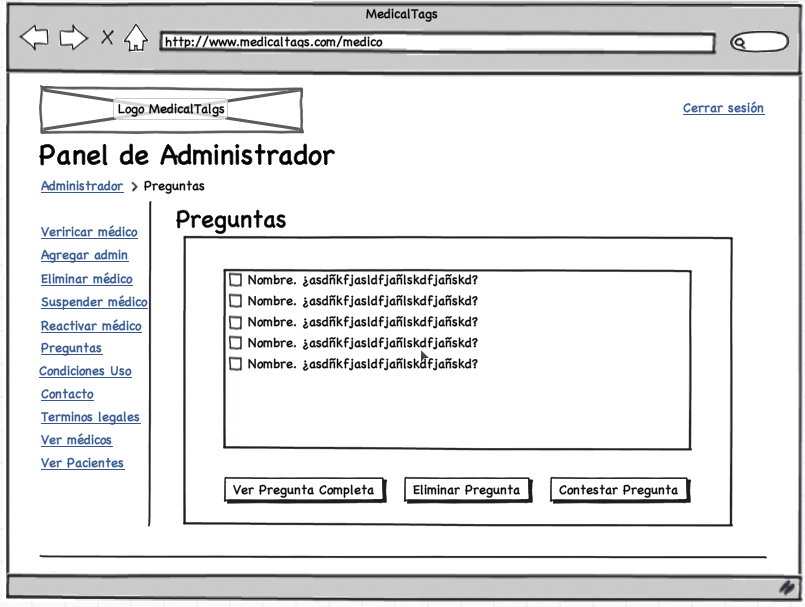
\includegraphics[width=12cm]{img/png/interfaz/99_Administrador.png}
		%  \caption{Panel de Administrador. Preguntas.}
		%  \label{fig:iu_admin_preguntas}
		%\end{figure}
	
	
		% section grafico (end)
\end{document}
% chapter diseño (end)